\chapter{Parallelization and Scaling}
\label{chap:Parallelization and Scaling}
We find the ability to parallelize and utilize available hardware important when designing a high-performance system for OLAP workloads. For ultimate performance, a system must be parallelized on all levels:

\begin{itemize}
  \item Utilize computing power in a distributed, share-nothing environment.
  \item Utilize all sockets in a non-uniform memory access (NUMA) architecture.
  \item Exploit thread-level parallelism within a multicore processor.
  \item Exploit instruction-level parallelism within a single core.
  \item Use single input, multiple data (SIMD) instructions available in the processors.
\end{itemize}

Parallelization can be applied to support more users and larger datasets, not only to improve raw performance.

\newpage

\section{Distributed Architecture}
\label{sec:Distributed Architecture}
For performance reasons, a database may be distributed across multiple servers. We refer to this as a \textit{shared-nothing} architecture, as all communication between the servers in the cluster must explicitly be passed through the network \cite{DeWitt1992-ki}. Some operations allow servers to process data locally and send processed and filtered results back to the client. Such operations are scalable since network traffic is reduced. Other operations are hard to perform on a distributed architecture, as it requires a substantial amount of inter-server processing. An example of such operation is \textit{join}.


Several of the systems studied in this research support a distributed architecture. Among them are \oracle~\cite{Mukherjee2015-ul}, \cstore~\cite{Stonebraker2005-qz}, \saph~\cite{Farber2012-vh} and \exasol~\cite{Exasol2014-xh}. These systems distribute data across nodes in the cluster, such that a single query usually must be executed on multiple servers and merged before sent back to the client.

\afigure{img/oracle-distributed.png}{\oracle~in-memory compression units (IMCUs) distributed across different nodes in a shared-nothing architecture. A page structure persists tables to disk, and the tables are brought up into memory as IMCUs. Different colors in the figure represent which IMCUs belong to which node in the cluster. Courtesy of \cite{Mukherjee2015-ul}.}{fig:oracle-distributed}{0.7}
In Section \ref{sec:Horizontal Partitioning}, we saw that \oracle~horizontally partitions the columns into in-memory compression units (IMCUs). In a distributed environment, these IMCUs can be spread across different nodes \cite{Mukherjee2015-ul}, as seen in Figure \ref{fig:oracle-distributed}. \oracle~supports distributed SQL execution, where a central query engine coordinates query execution across nodes in the cluster. 

The blocks in \oracle~are distributed using a two-phase strategy \cite{Mukherjee2015-ul}. First, a centralized coordination phase is performed such that servers can reach a minimal consensus. Second, IMCUs are distributed over the network in a decentralized manner. \oracle~in a distributed environment can be configured to be both \term{1-safe} and \textit{(N-1)-safe}.

\qlikview, one of the studied reference products, also supports a distributed architecture \cite{Qlik2012-ku}. We saw in Section \ref{sec:Business Discovery} that \qlikview~uses the definition of \textit{an application}, where an application is one or more \bd~panels connected to a specific data extract. An application is also the minimum distribution unit in \qlikview, which in practice means that a request belonging to an application will be handled by a single server.  In other words, \qlikview~in a distributed environment does not need a central coordination unit to merge results before sent back to the client.

In \qlikview, a single application might still be served by multiple machines \cite{Qlik2012-ku}. A load balancer will assign a user session to one of the servers in the cluster, such that all requests from that session are directed to the same server. Hence, two users running the same application might have different servers processing the requests.

\subsection{Column Distribution}
\label{sub:Column Distribution}

\ffigure{img/dictionary-scale-out}{Different data placements of a dictionary encoded column with an inverted index. \textit{IV} is the index vector, or the actual data column, containing dictionary keys. \textit{Dict} is the dictionary, while \textit{IX} is an inverted index structure. Each color represents a node in the cluster. Courtesy of \cite{Psaroudakis2015-lc}.}{fig:dictionary-scale-out}

We have previously pointed out the potential of dictionary encoded column storage for analytical workloads. Psaroudakis \ea~have studied three techniques of how such layout with inverted indexes can be distributed in a shared-nothing architecture \cite{Psaroudakis2015-lc}. These techniques are \textit{round-robin}, \textit{index vector partitioning}, and \textit{physically partitioning}, all which are illustrated in Figure \ref{fig:dictionary-scale-out}. The distribution assumes an \textit{Index Vector} (IV), which contains the dictionary encoded column values, a dictionary (Dict), and an optional inverted index structure (IX). The techniques comes with different benefits and disadvantages that we enumerate below.

\subsubsection{Round-robin (RR)}
\label{ssub:Round-robin (RR)}
RR the simplest form of data placement, where whole columns are placed on a single node in the cluster. This way, all scans and lookups on the column can happen locally. Columns are assigned a node in the cluster in a round-robin fashion.

RR does not account very well for data skew and fails to utilize the processing power of a cluster. A node might end up with one or more hot columns, which results in that node becoming the bottleneck of query execution.

\subsubsection{Index-Vector Partitioning (IVP)}
\label{ssub:Index-Vector Partitioning (IVP)}
IVP is a range-based partitioning of the data. In this distribution scheme, the columns (IV) are partitioned and spread across nodes in the cluster. This scheme accounts for data skew and better utilizes all nodes in a system.

Using IVP, there is no clear choice how to place the dictionary and the index structure. Psaroudakis \ea~suggest that interleaving these structures across all nodes averages out the latency. 

IVP suffers from poor performance on high-selectivity scans and index lookups due to excessive communication between nodes on dictionary and index lookup. The more nodes in the cluster, the larger this overhead gets.

\paragraph{Physically Partitioned (PP)}
\label{par:Physically Partitioned (PP)}
PP address the challenges with IVP by keeping local dictionaries and index structures per partition. The column values (IX) are still partitioned by range the same way as in IVP. This technique distributes work evenly across nodes in the cluster, and allows for data pruning based on minimum and maximum values, a technique we discussed in Section \ref{sec:Database Statistics}. Database systems using PP include \oracle~and \saph.

There are two main disadvantages with PP. First, it requires more computational resources to construct a local dictionary per partition instead of a global dictionary. Besides, column repartitioning requires dictionaries to be rebuilt. Second, since dictionaries across partitions are expected to contain common values, PP potentially consumes more memory.

\section{Thread-Level Parallelism}
\label{sec:Thread-lever Parallelism}
Within a single multiprocessor, where all processing units share memory, parallelization can be performed by using threads. Ideally, queries should use all available cores, and the ultimate goal is that query performance increases linearly with the number of processing units available. Conceptually, parallelization is simple: Partition the input onto the available processing units and merge the results after computation is done \cite{Neumann2011-uq}. In reality, some database operations can be tricky to implement in parallel. Besides, special care should be taken in which memory are accessed in a non-uniform memory access (NUMA) architecture.

Most modern database management systems use thread-level parallelism to improve performance. Systems here include \vertica~\cite{Lamb2012-kg}, \mssql~\cite{Larson2013-mc}, \blink~\cite{Barber2012-xt, Johnson2008-cp}, and \saph~\cite{Farber2012-vh}. \exasol, the top performing system on the TPC-H benchmark, applies parallelism on every layer, which includes thread-level parallelism \cite{Exasol2014-xh}. As for reference products in our research, both \qlikview~and \tableau~have reported that they scale almost perfectly with the addition of more processing units \cite{Kamkolkar2015-iq, Qlik2011-ef}. 

% paragraph explaining how each system splits queries
\blink~parallelizes SQL queries by breaking them up into \term{single-table queries} (STQ) that belongs to a column partition \cite{Barber2012-xt}. Each STQ is divided into blocks which are processed by threads in a thread pool. Since some partitions will be heavier to process, threads that finish their partition early will help the heavier-loaded threads by "stealing" some unprocessed blocks. We refer to the technique where idle threads "steal" tasks from active threads as \textit{work stealing}. 

\mssql~works similar to \blink. In this system, queries are divided into batches and processed in parallel by all threads in the system \cite{Larson2013-mc}.

% paragraphs illustrating the main challenges with parallelization and techniques used to fix it
The barriers for linear speedup are startup costs, interference and communication, and uneven distribution of work (data skew) \cite{DeWitt1992-ki}. In other words, the primary challenges in query processing are work distribution and scheduling \cite{Neumann2011-uq}. Besides, parallel joining and grouping/aggregation are not trivial to do in parallel.

\subsection{Scheduling}
\label{sub:Scheduling}
Psaroudakis \ea~have studied the details of thread scheduling \cite{Psaroudakis2013-fn}. Their research highlight three important things that must be considered when scheduling threads:
\begin{enumerate}
  \item The responsibility of scheduling cannot be given to the operating system (OS). If the OS is responsible for scheduling threads, severe overhead must be expected due to high creation costs and several context switches. Time sharing policies implemented in the OS are also sub-optimal for database workloads.
  \item A single thread pool should manage all threads in the system. \saph~uses three different thread pools: (i) dispatcher threads for partitioning queries, (ii) executor threads for SQL execution, and (iii) receiver threads that process network requests. The independence of the thread pools poses a problem since there exists no shared structure that keeps track of how many cores are actually in use.
  \item The state of the whole system should be taken into consideration when deciding task granularity. When a task divides itself into smaller subtasks, the number of subtasks created should be dependent on how many processing cores that are available at the time. A simplified example is if six out of eight processing units are busy, a task should only generate two subtasks instead of eight.
\end{enumerate}

\ffigure{img/scheduler.png}{Data structures used by a task scheduler. Each DAG represents a query. When a query is added to the task scheduler, the root node is put into a queue that corresponds to that query's priority. Courtesy of \cite{Psaroudakis2013-fn}.}{fig:scheduler}
A directed acyclic graph (DAG) can represent a parallelizable query where each node is a separate task that can be executed by a single thread \cite{Psaroudakis2013-fn}. Each thread can pick any task from the DAGs where the predecessor has already been processed. Also, task priorities can be supported by having a queue and a task pool per priority. Figure \ref{fig:scheduler} depicts the structures used by the scheduler.

Using the method described in the above paragraph, changing the probability that a root node (new query) is selected can adjust the throughput/latency tradeoff. If the probability of picking a root node is high, multiple queries execute simultaneously, and simpler queries might complete before heavier queries even though they were submitted at a later time. Hence, latency is reduced. If the probability of picking a root node is low, started queries normally finish before execution of new queries start. In this situation, throughput is maximized, but it comes at the cost of higher latency for simpler queries.

A system known to implement such task-based scheduling discussed in this section is \hyrise~\cite{Schwalb2014-hn}. In this system, all partitionable operators are split dynamically into tasks at runtime, and the size of the tasks are determined based on system parameters and the input size of the data. \hyrise~reports almost perfect load balancing. 

\subsection{NUMA Awareness}
\label{sub:NUMA Awareness}
\afigure{img/numa.png}{Representation of NUMA nodes. Accessing RAM local to a CPU is faster than accessing RAM that belongs to another processor. Courtesy of \cite{Qlik2013-an}.}{fig:numa}{0.7}
Non-Uniform Memory Access (NUMA) is a multiprocessor memory architecture designed to overcome the scalability limits of other known architectures \cite{Qlik2013-an}. As illustrated in Figure \ref{fig:numa}, a NUMA machine consists of several sockets where each socket has a multicore processor and local memory. Communication between sockets is done over an interconnection network. In other words, memory in NUMA machines are decentralized, so communication costs between the different sockets must be taken into consideration when making parallelization decisions \cite{Psaroudakis2015-lc}. A database that runs on a NUMA architecture should be aware that not all memory can be accessed with the same latency. A scheduler that is \textit{NUMA aware} can have up to 5x performance compared to a scheduler that is not.

We saw that \blink~uses \term{work stealing} among threads, a technique known to increase database performance \cite{Barber2012-xt}. However, in a NUMA architecture, \textit{work stealing} might hurt performance. Psaroudakis \ea~distinguish between memory-intensive and CPU-intensive tasks \cite{Psaroudakis2015-lc}. If a memory-intensive task is stolen across a socket in a NUMA architecture, throughput can be hurt up to 58\%. To keep track of which socket a task belongs to, a page socket mapping structure can be used.

An example of a NUMA aware system is \hyper~\cite{Psaroudakis2014-ma, Psaroudakis2015-lc}. \hyper~distributes works across sockets,  uses task stealing, and exploits elastic parallelism. Data locality is optimized. In this system, tasks are divided into two classes: Memory intensive and CPU intensive. Memory intensive tasks should not be stolen across sockets, but this is allowed for CPU intensive tasks.

The \qlikview~developers conclude that NUMA is great if the application can take advantage of it \cite{Qlik2013-an}. However, if it does not, NUMA might have a negative impact on performance. \qlikview~actually performs better if NUMA is disabled in BIOS. When NUMA is disabled, the operating system will use the local memory for one CPU at a time.

We conclude this section by emphasizing the fact that techniques developed for distributed, shared-nothing architectures (Section \ref{sec:Distributed Architecture}) can be used to enhance performance on NUMA nodes \cite{Mukherjee2015-ul}. Each socket in a NUMA architecture can be treated as a single server in a shared-nothing architecture such that all communication is performed with explicit message passing. The column distribution schemes we discussed in Section \ref{sub:Column Distribution} can also be applied to a NUMA system, both in a shared-memory and shared-nothing architecture.

\subsection{Hyperthreading}
\label{sub:Hyperthreading}
Hyperthreading is a technique implemented in modern CPUs to improve parallelization of computations \cite{Wikipedia_contributors2015-yx}. For each physical core in the processor, the operating system addresses two logical cores. The core function of hyperthreading is to increase the number of independent instructions to utilize the potential of super-scalar processors. It also helps with closing the \textit{memory gap}, which means the processor is better utilized when executing threads that are memory-bound. Hyperthreading can be used to speed up certain database operations, like the probe phase in joins \cite{Barber2014-ey}.

However, if a single thread manages to keep a processing core busy with computations, hyperthreading will degrade performance due to unnecessary context switching and overhead. A whitepaper from \qlikview~says that hyperthreading should be disabled for maximum performance \cite{Qlik2011-yc}.

\section{Instruction Level Parallelism}
\label{sec:Instruction Level Parallelism}

Instruction-level parallelism (ILP) can be exploited if a processor can find operations that are independent \cite{Wikipedia_contributors2015-vg}, as it allows a processor to execute multiple instructions simultaneously. Techniques that allow multiple operations to be executed at the same time include \term{instruction pipelining} and \term{superscalar execution}. As most programming languages do not require application programmers to specify which instructions are independent, exploiting ILP is the job of the compilers and processors.

It is still possible to implicitly design applications that are optimized for ILP. In general, the idea is that if a processor can find enough independent work, it can be one or two magnitudes faster \cite{Boncz2005-wj}. Techniques used to reduce dependencies between instructions include \textit{branch avoidance} and \textit{loop pipelining}, which we study further in Chapter \ref{chap:Hardware Utilization}.

\section{SIMD}
\label{sec:SIMD}
\afigure{img/simd.png}{SIMD execution model: In (a) scalar mode: one operation produces one result. In (b) SIMD mode: one operation produces multiple results. Courtesy of \cite{Willhalm2009-hu}.}{fig:simd}{0.8}
% Present problem
Within a single execution context, instructions that work on multiple elements at a time can be used to increase query performance. We refer to these instructions as single input, multiple data (SIMD) instructions \cite{Wikipedia_contributors2015-ax}. As seen in Figure \ref{fig:simd}, an SIMD instruction applies the same operation to multiple operands simultaneously. SIMD processing in a database context is particularly effective if we can keep an entire processing block in the CPU registers \cite{Neumann2011-uq}, and Willhalm \ea~show that SIMD processing using a vectorized model can be up to 1.5 times faster than databases optimized for scalar execution and ILP \cite{Willhalm2009-hu}.

Our research shows that several database systems use SIMD parallelization. Systems in this category include \oracle~\cite{Lahiri2015-mz}, \blink~\cite{Barber2012-xt}, and \ibm~\cite{Raman2013-em}. A whitepaper from the developers of \exasol~says that SIMD features of modern processors must be used to reach the highest level of performance \cite{Exasol2014-xh}.

\afigure{img/oracle-simd.png}{Filter operation in \oracle~using SIMD vector processing. Courtesy of \cite{Lahiri2015-mz}.}{fig:oracle-simd}{0.6}
\oracle~performs scans against the columns using instructions that work on multiple operands simultaneously \cite{Lahiri2015-mz}. As seen in Figure \ref{fig:oracle-simd}, a filter operation benefits from SIMD as multiple values can be compared in parallel. \ibm~and later versions of \blink~work similarly \cite{Barber2012-xt, Raman2013-em}.

\begin{figure}
  \centering
  \begin{subfigure}{0.45\textwidth}
    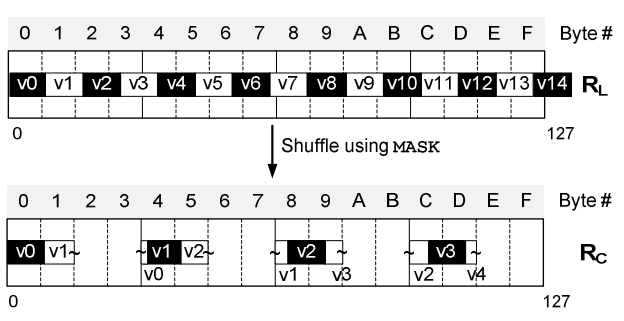
\includegraphics[width=\textwidth]{img/simd-align-1.png}
    \caption{Using a \texttt{MASK} operation to align values to data words.}
    \label{fig:simd-align-1} 
  \end{subfigure}
  \begin{subfigure}{0.45\textwidth}
    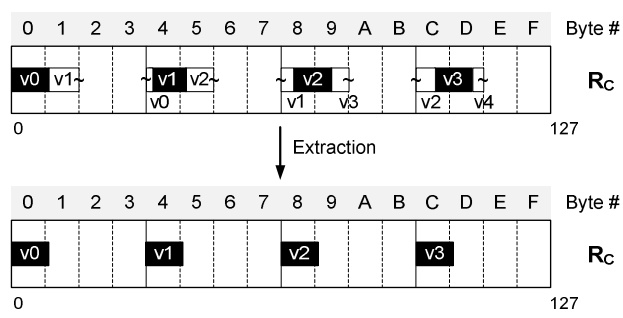
\includegraphics[width=\textwidth]{img/simd-align-2.png}
    \caption{Extracting values by bitshifting followed by masking out irrelevant bits.}
    \label{fig:simd-align-2} 
  \end{subfigure}
  \caption{Aligning a bitpacked vector for SIMD execution. Courtesy of \cite{Willhalm2009-hu}.}
  \label{fig:simd-align} 
\end{figure}

Bitpacking of column values further increase SIMD performance, because more values fit within a single data word. However, since most SIMD instructions require operands to be aligned, some preprocessing steps must be applied to the column values first \cite{Willhalm2009-hu}. As seen in Figure \ref{fig:simd-align}, a bitpacked vector can be prepared for an SIMD operation using mask and bitshift operations. Vectors that are already aligned with data words can be queried more efficiently since the preprocessing can be skipped.

Most literature refers to SIMD parallelization as utilizing special processor and instruction set extensions, like the Intel SSE and Intel AVX2 extension \cite{Willhalm2013-ri, Willhalm2009-hu}. However, general CPU instructions can also be used to evaluate predicates in a \textit{SIMD-like fashion}. In \blink, ordinary CPU instructions work directly on multiple values in a bitpacked column by applying a suitable mask and compare the result with a second mask containing the expected values \cite{Johnson2008-cp}. This technique can become very efficient since masks for a column are calculated once per query.

\section{Scaling}
\label{sec:Scaling}
\textit{Scaling} is action taken to accomodate more work in a computer system \cite{Wikipedia_contributors2015-lw}. Scaling can be used to support more users and handle larger datasets while keeping performance at an acceptable level. In a \bd~setting, scaling is necessary because data volumes are becoming increasingly larger \cite{Qlik2012-ku}.


\afigure{img/scaling.png}{Scale-Up vs Scale-Out. When scaling up, more hardware is added to the single server. When scaling out, more servers are added. Courtesy of \cite{CloudBoost2015-gg}.}{fig:scaling}{0.8}
We distinguish between two types of scaling, as seen in Figure \ref{fig:scaling}. \textit{Scaling up} refers to scaling by adding more hardware to a single server. Examples of hardware improvement are the addition of more RAM or more processing cores. \textit{Scaling out} refers to the technique where the system scales by adding more servers to a processing cluster. A system that allows for scaling out must be built using a distributed architecture, as we explained in Section \ref{sec:Distributed Architecture}.

Whether to scale out or scale up is discussed by Mukherjee \ea~\cite{Mukherjee2015-ul}. Historically, scaling out has been considered as the best and most flexible way to achieve good performance. Scaling out is strictly required for very large systems, since there is a limit of how much processing power and storage capacity a single server can provide. Scaling out also comes at the benefit of redundancy; if one node in the cluster goes down, another node can take over.

However, there are situations where scaling up should be considered. First of all, a shared-memory application is easier to program than a shared-nothing, distributed application \cite{Boncz2002-yj}. Second, if results and queries are cached, it is beneficial that all requests are handled by the same server. \qlikview~reports that scaling up is up to twice as fast as scaling out for a large application with many users due to the effects of caching \cite{Qlik2012-ku}.

We conclude this section by saying that if the dataset is small enough to fit on a single server, scaling up should be considered over scaling up, due to simpler implementation and better cache utilization. It is indeed likely that the datasets actually are small enough to fit on a single server. 80\% of Facebooks tasks are less than 10GB \cite{Mukherjee2015-ul}, and all of Amazon's transactions for a year takes up roughly 50 GB \cite{Kemper2011-ap}.

\section{Chapter Conclusion}
\label{sec:Chapter Conclusion}
We conclude this chapter by saying that parallelization is an important measure to improve a \bd~application's performance and that it might be required to handle large data sizes and multiple users. Many systems studied in this research use parallelization, including \exasol, \tableau, and \qlikview.

We recommend utilizing thread-level parallelism, where queries should be split into smaller tasks and executed by threads in a thread pool. It is important for the scheduler to distribute work evenly to get linear speedup.

Instruction level parallelism and SIMD instructions are both promising techniques to improve database performance. We see that SIMD instructions are particularly effective on bitpacked columns, a storage format we have suggested earlier in this report. The database software should also be designed to improve ILP. We will study ILP in detail in the chapter about hardware utilization, Chapter \ref{chap:Hardware Utilization}.

For now, we do not recommend a distributed architecture, because of three reasons. First, a distributed architecture is harder to program than an application that runs on a single server. Second, distributed queries might hurt query cache performance, as reported by \qlikview. Last, we anticipate that most workloads fit in the main memory of a single server. For the same three reasons, we encourage a \textit{scale up} approach to scaling instead of \textit{scale out}. However, if a single server is no longer cabable of handling all incoming requests, we recommend scaling out like \qlikview~by distributing full data extracts and \bd~panels across different servers.
